% !TEX program = xelatex
\documentclass{beamer}
\usepackage{beamerthemeDuke} 
\usepackage{tcolorbox}
\usepackage{multicol}
\usepackage{graphicx}


\definecolor{lightcoral}{rgb}{0.94, 0.5, 0.5}
\definecolor{coralred}{rgb}{1.0, 0.25, 0.25}
\definecolor{classicrose}{rgb}{0.98, 0.8, 0.91}
% \definecolor{graphcolor}{rgb}{0.88, 0.91, 0.93}
\definecolor{americanrose}{rgb}{1.0, 0.01, 0.24}
\definecolor{graphcolor}{RGB}{235, 226, 232}
\setbeamercolor{block title example}{bg=PMS 166, fg=white}
\setbeamercolor{block body example}{bg=PMS 157!20, fg=PMS Black 3}
\definecolor{aliceblue}{rgb}{0.94, 0.97, 1.0}
\usetheme{Duke}
\setbeamercovered{transparent}

% Normal blocks
\setbeamercolor{block title}{bg=Duke Blue, fg=white}
\setbeamercolor{block body}{bg=aliceblue!95!black, fg=PMS Black 3}

% Alert blocks
\setbeamercolor{block title alerted}{bg=lightcoral, fg=white}
\setbeamercolor{block body alerted}{bg=aliceblue!95!black, fg=PMS Black 3}

% Example blocks
\setbeamercolor{block title example}{bg=Blue Devil Blue, fg=white}
\setbeamercolor{block body example}{bg=aliceblue!95!black, fg=PMS Black 3}

% Strength blocks

\definecolor{indiagreen}{rgb}{0.07, 0.53, 0.03}
\setbeamercolor{block title strength}{bg=indiagreen, fg=white}
\setbeamercolor{block body strength}{bg=aliceblue!95!black, fg=PMS Black 3}

\newenvironment{strengthblock}[1]{%
  \begin{beamerboxesrounded}[upper=block title strength,lower=block body strength]{#1}%
}{%
  \end{beamerboxesrounded}%
}

% Weakness blocks
\definecolor{officegreen}{rgb}{0.0, 0.5, 0.0}
\setbeamercolor{block title weakness}{bg=orange, fg=white}
\setbeamercolor{block body weakness}{bg=aliceblue!95!black, fg=PMS Black 3}

\newenvironment{weaknessblock}[1]{%
  \begin{beamerboxesrounded}[upper=block title weakness,lower=block body weakness]{#1}%
}{%
  \end{beamerboxesrounded}%
}

\setbeamertemplate{blocks}[rounded][shadow=false]


% ---- force white everywhere ----
\setbeamercolor{background canvas}{bg=white}
\setbeamercolor{normal text}{bg=white}
\setbeamercolor{sidebar}{bg=white}
\setbeamercolor{palette sidebar primary}{bg=white}
\setbeamercolor{palette sidebar secondary}{bg=white}
\setbeamercolor{palette sidebar tertiary}{bg=white}
\setbeamercolor{palette sidebar quaternary}{bg=white}

% \usecolortheme{Duke}
% \usepackage{bookman}
% \usefonttheme{serif} % Or serif
\setbeamercovered{transparent}



%Information to be included in the title page:
\title[Cell Multiprocessor] %optional
{Introduction to the \\ \textbf{Cell Multiprocessor}}




\date[2005] % (optional)
{Kahle, Day, Hofstee, Johns, Maeurer, Shippy \\ \textit{Sony} + \textit{IBM} + \textit{Toshiba}}

\author[\today] % (optional, for multiple authors)
{Roshan Sundaram}



\begin{document}

\frame{\titlepage}


% Background
\begin{frame}
\frametitle{Background}
\begin{tcolorbox}[colback=blue!5!white,colframe=blue!75!black]
  \begin{center}

  Time for a \textbf{next-generation PlayStation} gaming console. \\
  \begin{itemize}
    \item \textit{Sony} provides content (for games) 
    \item \textit{IBM} develops the microprocessor 
    \item \textit{Toshiba} manufactures the chip
  \end{itemize}
  \end{center}


\end{tcolorbox}

\only<2>{\begin{tcolorbox}[colback=indiagreen!30!white,colframe=indiagreen!75!black]
  \begin{center}
    What do you do with \\ 
  \LARGE \$400,000,000???
  \end{center}
\end{tcolorbox}
}

\end{frame}


% Why Cell?
\begin{frame}
\frametitle{Motivation}

\begin{tcolorbox}[colback=blue!5!white,colframe=blue!75!black]
  \begin{center}


  Sony wanted \textbf{100x the performance} of the PlayStation2
  \end{center}

\end{tcolorbox}




Three main limiters of performance:
\begin{enumerate} 
  \item Memory latency and bandwidth
  \item Power density and cooling
  \item High-frequency \& pipelining
\end{enumerate}

\begin{tcolorbox}[colback=PMS 166!15!white,colframe=PMS 166!100!white]
    \begin{center}
      \textbf{Solution:} design a custom CPU from scratch, using cutting-edge technologies
    \end{center}
  \end{tcolorbox}



\end{frame}

% Challenges
\begin{frame}
\frametitle{Challenges}

This ambitious approach had several obstacles to overcome\dots 

\begin{alertblock}{High-Bandwidth Communication}
  Need an architecture that maximizes in-flight memory transactions
\end{alertblock}

\begin{alertblock}{Power Efficient}
  Device must be efficient, cool, and compact 
\end{alertblock}

\begin{alertblock}{Exploit Parallelism}
  Find new parallelism outside of high-performance OoO cores
\end{alertblock}

\textit{Also: support internet features and make the design modular\dots}






\end{frame}



% The main issue
\begin{frame}
\frametitle{Design Goals}

Ten main outlined goals:

\begin{table}
  \centering
  \begin{tabular}{|c|c|}
    \hline
    High design frequency & Power Architecture  \\
    \hline
    SIMD operation & Efficient PPE core \\
    \hline
    SPEs with local memory & High-bandwidth I/O \\
    \hline
    Custom implementation & Test \& Debug Support \\
    \hline
    Low-cost packaging & Low-power transistors \\
    \hline
  \end{tabular}
  \end{table}


\begin{tcolorbox}[colback=PMS 166!15!white,colframe=PMS 166!100!white]
    \begin{center}
      High-throughput \textbf{vectorized processor} that is power-efficient and low-cost
    \end{center}
  \end{tcolorbox}


\end{frame}



% Framework
\begin{frame}
\frametitle{Hardware Overview}

\begin{itemize} 
  \item Power ISA chip with a big core (PPE) and 8 small cores (SPEs)
  \item Use \textbf{direct memory access} for inter-element communication
\end{itemize}

\begin{multicols}{2}

\begin{tcolorbox}[colback=blue!5!white,colframe=blue!75!black]
  \begin{center}
    \textbf{One Big Core}
  \end{center}
\end{tcolorbox}

\columnbreak

\begin{tcolorbox}[colback=classicrose!50!white,colframe=classicrose!35!black]
  \begin{center}
    \textbf{Eight Small Cores}
  \end{center}
\end{tcolorbox}

\end{multicols}

\begin{tcolorbox}[colback=graphcolor,colframe=graphcolor!75!black]
  \begin{center}
    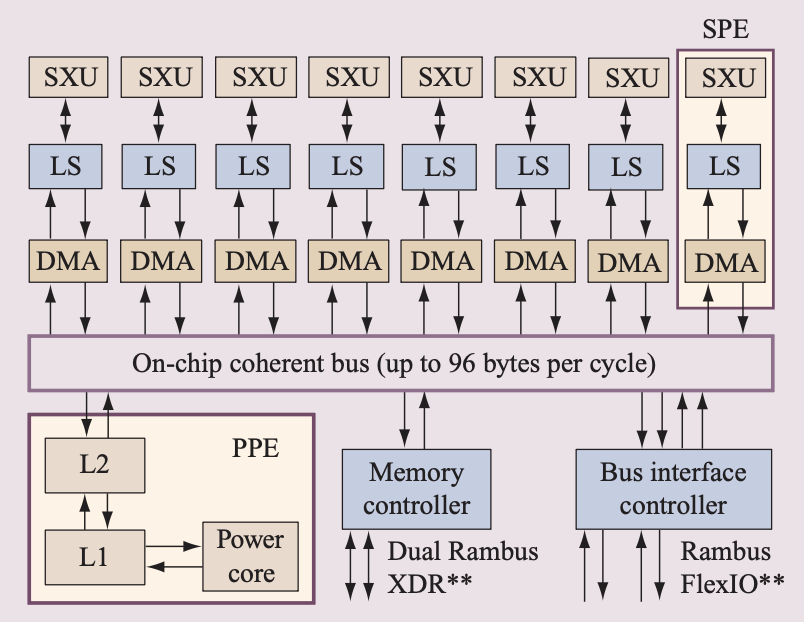
\includegraphics[width=0.5\textwidth]{CellBlockDiagram.png}
  \end{center}
\end{tcolorbox}



\end{frame}

\begin{frame}
  \frametitle{Big Core: Power Processing Element}
  \begin{itemize}
    \item Dual-issue superscalar, in-order, 2-way multithreading 
    \item Internal hierarchical cache and regfile
    \item Fetch, decode, branch, issue, completion
    \item Basic arithmetic
  \end{itemize}

\begin{tcolorbox}[colback=graphcolor,colframe=graphcolor!75!black]
  \begin{center}
    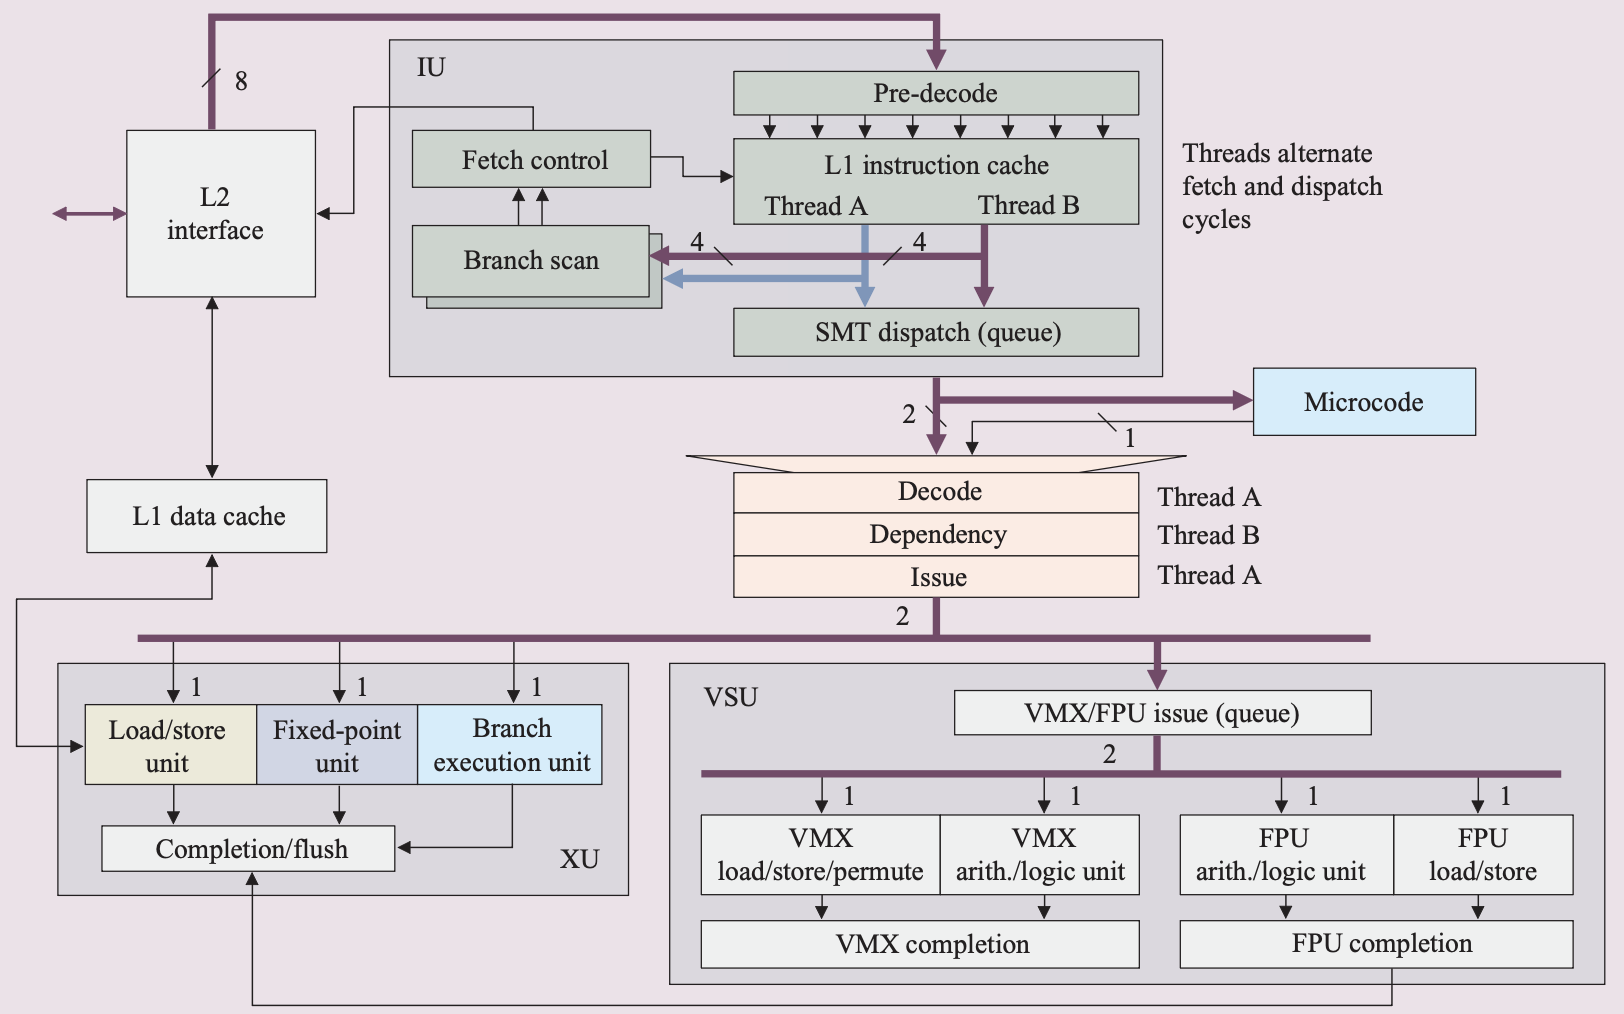
\includegraphics[width=0.7\textwidth]{PPEDiagram.png}
  \end{center}
\end{tcolorbox}

\end{frame}


% Roofline Description
\begin{frame} 
  \frametitle{Small Core: Synergistic Processing Element}
  \begin{itemize}
    \item Optimized for compute-intensive and media applications
    \item Shares address space with PPE and uses DMA but cannot directly access main memory
    \item Overcomes the ``memory wall'' by allowing many in-flight memory transactions 
    \item Designed for SIMD workloads (vectors only) 
    \item \textbf{No cache!!!} Only 256 KB of local scratchpad memory
  \end{itemize}

\begin{tcolorbox}[colback=graphcolor,colframe=graphcolor!75!black]
  \begin{center}
    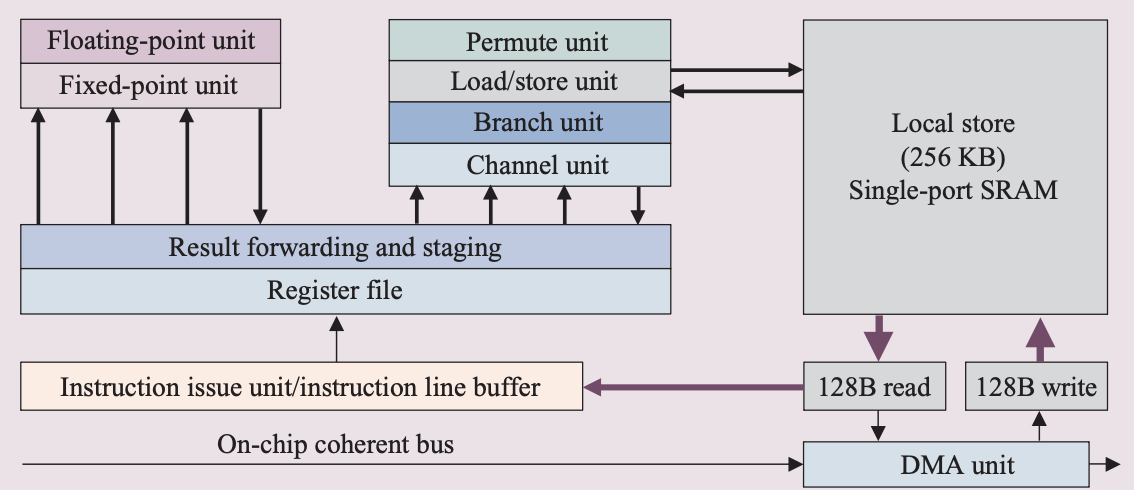
\includegraphics[width=0.7\textwidth]{SPEDiagram.png}
  \end{center}
\end{tcolorbox}

  
\end{frame}



\begin{frame} 

  \frametitle{A Unique Design!}
  What is so special about the Cell architecture?
  \begin{itemize}
    \item PPE used for control, \textbf{SPEs do the heavy-lifting}
    \item Hides latency with \textbf{concurrency} instead of speculation
    \item \textbf{Fast on-chip bus} for efficient DMA (96 B/cycle)
    \item High-bandwidth DRAM interface (25.6 GB/s)
  \end{itemize}
  
  Also used \textbf{advanced fabrication techniques}:
  \begin{itemize} 
    \item Low-Cost packaging with high I/O bandwidth (85 GB/s)
    \item Silicon on insulator transistors for improved power efficiency
  \end{itemize}

  % \begin{multicols}{2}

  % \begin{tcolorbox}[colback=blue!5!white,colframe=blue!75!black]
  %   \begin{center}
  %     \textbf{Low-Cost Packaging with high I/O bandwidth}
  %   \end{center}
  % \end{tcolorbox}

  % \columnbreak

  % \begin{tcolorbox}[colback=classicrose!50!white,colframe=classicrose!35!black]
  %   \begin{center}
  %     \textbf{Silicon on Insulator transistors for power efficiency}
  %   \end{center}
  % \end{tcolorbox}

  % \end{multicols}


\end{frame}





% Parameter 3 Information 
\begin{frame} 
  \frametitle{Hardware Oddities}

  \begin{exampleblock}{Heterogeneous Design}
    PPE functions as a normal core, but SPEs can be used flexibly 
    
  \end{exampleblock}

  \begin{exampleblock}{Scratchpad Memory}
    Cacheless design requires programmer to move data around.  \\
    Not constrained by a hierarchical memory system (or cache misses). 
    
  \end{exampleblock}

  \begin{alertblock}{Programming Flexibility} 
    Software engineers can adapt SPEs to meet their needs\dots \\

  \end{alertblock}

\end{frame}

% Evaluation Benchmarks

\begin{frame}
  \frametitle{Using Cell}

  To exploit novel hardware, your code must be \textbf{optimized}, so\dots 
  \begin{tcolorbox}[colback=indiagreen!15!white,colframe=indiagreen!75!black]
   \begin{center} 
      \textbf{Goal:} make programming Cell as easy as possible 
   \end{center}
  \end{tcolorbox}

  \begin{tcolorbox}[colback=PMS 166!15!white,colframe=PMS 166!100!white]
    \begin{center}
      \textbf{Challenge:} explicitly managing local memories is hard
    \end{center}
  \end{tcolorbox}

  \begin{itemize}
    \item DMA currently handled by programmer $\rightarrow$ later by compiler?
    \item Vector processing unlocks lots of performance!
    \item \textbf{Must use SPEs} to maximize performance \& efficiency of Cell
  \end{itemize}
\end{frame}

% Programming models, part 1

\begin{frame}
  \frametitle{Programming Models}

  \begin{exampleblock}{Functional Offload}
    SPEs act as accelerators for library calls. \\
    Main program runs on PPE $\rightarrow$ outsource work to SPE. \\
    {\color{indiagreen} Main program logic is unchanged.}
  \end{exampleblock}

  \begin{exampleblock}{Computational Acceleration}
    PPE acts as a controller\dots SPEs do the processing. \\ 
    Must efficiently schedule DMA ops. for correct data movement. \\
    {\color{indiagreen} Accelerate complex math functions without rewriting apps.}
  \end{exampleblock}

  \begin{exampleblock}{Streaming}
    ``Pipelining'' computation with message passing. \\
    Each SPE applies a kernel then passes on the work. PPE controls. \\
    {\color{indiagreen} Each step should do equal work.}
  \end{exampleblock}
  
\end{frame}

% Programming models, part 2
\begin{frame}
  \frametitle{More Programming Models}

  \begin{exampleblock}{Device Extension}
    SPEs emulate a hardware device. \\
    PPE communicates via queues and registers. \\
    SPE can run in an isolated environment. \\
    {\color{indiagreen} Digital Rights Management.}
  \end{exampleblock}

  \begin{exampleblock}{Shared-Memory Multiprocessor}
    Similar to a shared-memory chip with atomic ops. \\
    SPEs uses DMA, PPE uses loads/stores.  \\
    {\color{indiagreen} Behaves (somewhat) like other shared-memory processors. }
  \end{exampleblock}

  \begin{exampleblock}{Asymmetric Thread Runtime}
    Threads run on PPE for general tasks or SPEs for compute. \\
    OS schedules tasks on PPE and SPEs based on program demands. \\
    {\color{indiagreen} Moves the burden of scheduling to software.}
  \end{exampleblock}
  
\end{frame}


% Evaluation Results

% {
% \setbeamercolor{background canvas}{bg=graphcolor}
% \begin{frame}
%   \frametitle{Evaluation Results (Quantitative)}

%     \begin{table}
%       \centering
%       \begin{tabular}{|c|c|}
%         \hline
%         \includegraphics[width=0.45\textwidth]{BenchXeon.png} &
%         \includegraphics[width=0.45\textwidth]{BenchOpteron.png} \\
%         \small Intel Xeon &
%         \small AMD Opteron \\
%         \hline
%         \includegraphics[width=0.45\textwidth]{BenchSPARC.png} &
%         \includegraphics[width=0.45\textwidth]{BenchCell.png} \\
%         \small Sun UltraSPARC &
%         \small IBM Cell \\
%         \hline
%       \end{tabular}
%     \end{table}


%   \end{frame}
% }

% Evaluation Results qualitative
% \begin{frame} 
% \frametitle{Evaluation Results (Qualitative)}


% \end{frame}


% Strengths 
\begin{frame} 
\frametitle{Strengths}

\begin{strengthblock}{Vectors!!}
  Highlighted the importance of \textbf{SIMD} for games/media, especially as ILP reached its limits.
\end{strengthblock}

\vspace{3mm}

\begin{strengthblock}{Integrated Custom Design}
  Big \$\$\$ enabled software, architecture, and fabrication teams to build a \textbf{bespoke chip for PS3}.
\end{strengthblock}

\vspace{3mm}

\begin{strengthblock}{Flexible Programming Models}
  Users could \textbf{adapt the Cell} to whatever task they were doing (gaming, compute, clusters, etc.)\dots and they did!
\end{strengthblock}


\end{frame}

% Weaknesses 
\begin{frame} 
\frametitle{Weaknesses}

\begin{weaknessblock}{Painful to Program}
  \textbf{Managing memory manually is difficult}, and required developers to rewrite their code. 
\end{weaknessblock}

\vspace{3mm}

\begin{weaknessblock}{Lack of Compiler Support}
  Lack of strong compiler at release made DMA tricky for developers.   
\end{weaknessblock}

\vspace{3mm}

\begin{weaknessblock}{Poor Performance without SIMD}
  If your code didn't \textbf{use SPEs}, you were constrained by the PPE. 
\end{weaknessblock}

\vspace{3mm}
\begin{weaknessblock}{Vague ``Peak-Performance''}
  What does ``near-peak performance'' mean?
\end{weaknessblock}


\end{frame}


\begin{frame} 
  \frametitle{Cell's (Complicated) Legacy}

  \begin{tcolorbox}[colback=americanrose!15!white,colframe=americanrose!100!white]
    \begin{center}
      Cell was a \textbf{commercial failure}, but ahead of its time
    \end{center}
  \end{tcolorbox}
  \begin{itemize} 
    \item PlayStation 3 outsold competitor Xbox 360 (also a Power ISA)
    \item Cell processor only lasted one generation
    \item Developers didn't rewrite games to maximize Cell's potential
    \item Consoles moved to  AMD x86 chips 
  \end{itemize}

  \begin{tcolorbox}[colback=indiagreen!15!white,colframe=indiagreen!75!black]
   \begin{center} 
      Cell \textbf{paved the way for modern heterogeneous SoCs} with dedicated media accelerators -- like Apple Silicon \& big.LITTLE -- and GPUs. 
   \end{center}
  \end{tcolorbox}


\end{frame}


\begin{frame} 
\frametitle{Questions}


\begin{tcolorbox}[colback=blue!5!white,colframe=blue!75!black]
  How did Cell perform empirically? Did Sony benchmark it against other Power or x86 devices?
\end{tcolorbox}
\vspace{1mm}
\begin{tcolorbox}[colback=blue!5!white,colframe=blue!75!black]
  Of the various programming models, which was the most popular, and was this flexibility an impediment to development?
\end{tcolorbox}
\vspace{1mm}
\begin{tcolorbox}[colback=blue!5!white,colframe=blue!75!black]
  How well would Cell have scaled if the designers put more than 1 PPE and 8 SPEs on a single die? Is a chiplet-based approach feasible?
\end{tcolorbox}
\vspace{1mm}
\begin{tcolorbox}[colback=blue!5!white,colframe=blue!75!black]
  Why did GPUs succeed while Cell failed?
\end{tcolorbox}


\end{frame}



\end{document}